\documentclass{article}

\usepackage[utf8]{inputenc}
\usepackage[brazilian]{babel}
\usepackage{graphicx}
\usepackage{float}
\usepackage[pdftex]{hyperref}
\usepackage{epstopdf}
\usepackage{etoolbox}
\usepackage{amsmath}
\usepackage{amsfonts}
\usepackage{amssymb}
\usepackage{caption}
\usepackage{subcaption}
\usepackage{setspace}
\usepackage{tikz}

\patchcmd{\thebibliography}{\section*}{\section}{}{}
\newcommand{\R}{\ensuremath{\mathbb{R}}}
\newcommand{\Prob}{\ensuremath{\mathbb{P}}}
\newcommand{\K}{\ensuremath{\mathbb{K}}}
\newcommand{\U}{\ensuremath{\mathbb{U}}}
\newcommand{\N}{\ensuremath{\mathbb{N}}}
\newcommand{\Lg}{\ensuremath{\mathbb{L}}}
\newcommand{\T}{\ensuremath{\rm Tr}}
\newcommand{\sg}{{\sigma(x_k)}}

\newcommand{\G}{\ensuremath{\mathcal{G}}}
\newcommand{\F}{\ensuremath{\mathcal{F}}}
\newcommand{\C}{\ensuremath{\mathcal{C}}}
\newcommand{\E}{\ensuremath{\mathcal{E}}}
\newcommand{\Hn}{\ensuremath{\mathcal{H}}}
%\newcommand{\Hoo}{\ensuremath{\mathcal{H}_\infty}}
\newcommand{\Hop}{\ensuremath{\mathcal{H}_{op}}}
% --------------------------------------------------
\newtheorem{theo}{Teorema}
\newtheorem{exa}{Exemplo}
\newtheorem{lemm}{Lema}
\newtheorem{coro}{Corolário}
\newtheorem{defn}{Definição}[section]

%opening


\begin{document}

\begin{titlepage}
\begin{center}

\newcommand{\HRule}{\rule{\linewidth}{0.5mm}}
% Upper part of the page. The '~' is needed because \\
% only works if a paragraph has started.

\includegraphics[width=0.15\textwidth]{logounicamp.pdf}~\\[1cm]

\textsc{\LARGE Universidade Estadual de Campinas}\\[1.5cm]

\textsc{\Large Faculdade de Engenharia Mecânica}\\[0.5cm]

% Title
\HRule \\[0.4cm]
{ \huge \bfseries ES828 - Laboratório de Controle de Sistemas\\ \vspace{1cm} Relatório - Experimento 2 \\
\Large{Método de identificação de plantas eletrônicas} \\[0.4cm] }

\HRule \\[1.5cm]

% Author and supervisor
\begin{minipage}{0.6\textwidth}
\begin{flushleft} \large
\emph{Nome:}\\
Daniel Dello Russo Oliveira\\ Marcelli Tiemi Kian
\end{flushleft}
\end{minipage}
\begin{minipage}{0.2\textwidth}
\begin{flushright} \large
\emph{RA}\\ 101918\\
117892
\end{flushright}
\end{minipage}

\vfill

% Bottom of the page
{\large \today}

\end{center}
\end{titlepage}


\onehalfspacing
\section{Objetivos} 
O objetivo desse experimento é a familiarização com as ferramentas de design e simulação de sistemas de controle pelo Matlab e o estudo do projeto de controladores PID. 
	
\section{Projeto dos Controladores}
Consideramos a planta cuja função de transferência representada pela equação \ref{eq:gs} que foi obtida usando as medidas realizadas durante o experimento 2, consideramos também para todos os controladores uma envoltória $\epsilon = 2\%$. Cujos valores estão na tabela \ref{tab:valores}\\

\begin{equation}
\label{eq:gs}
G(s) = \frac{\kappa_1*\kappa_2*\kappa_3*\kappa_4}{(s*\tau_2 + 1)(s*\tau_3 + 1)s}
\end{equation}

\begin{table}[H]
\centering
\caption{Parâmetros numéricos da função de transferência}
\label{tab:valores}
\begin{tabular}{|c|c|}
	\hline Componente & Valor \\ 
	\hline $\kappa_1$ & $-0.1005$\\ 
	\hline $\kappa_2$ & $-2.1508$\\ 
	\hline $\kappa_3$ & $-4.6448$\\ 
	\hline $\kappa_4$ & $-5.6307$\\ 
	\hline $\tau_2$ & $0.0210$\\ 
	\hline $\tau_3$ & $0.0244$ \\ 	
	\hline 
\end{tabular} 
\end{table}

\subsection{Projeto do controlador proporcional}
Através do método do lugar das raízes, projetamos um controlador proporcional $C(s) = \kappa$ de forma a obter um tempo de estabilização mínimo, para isto inicialmente plotamos com o auxílio do Matlab o diagrama de lugar das raízes para a planta, que pode ser observado na figura \ref{fig:rlocusgs} e analisamos o tempo de estabilização do sistema para dois pontos que poderiam minimizar esse valor, um com amortecimento crítico e o outro com sobrelevação de $2\%$. 
\begin{figure}[H]
\centering
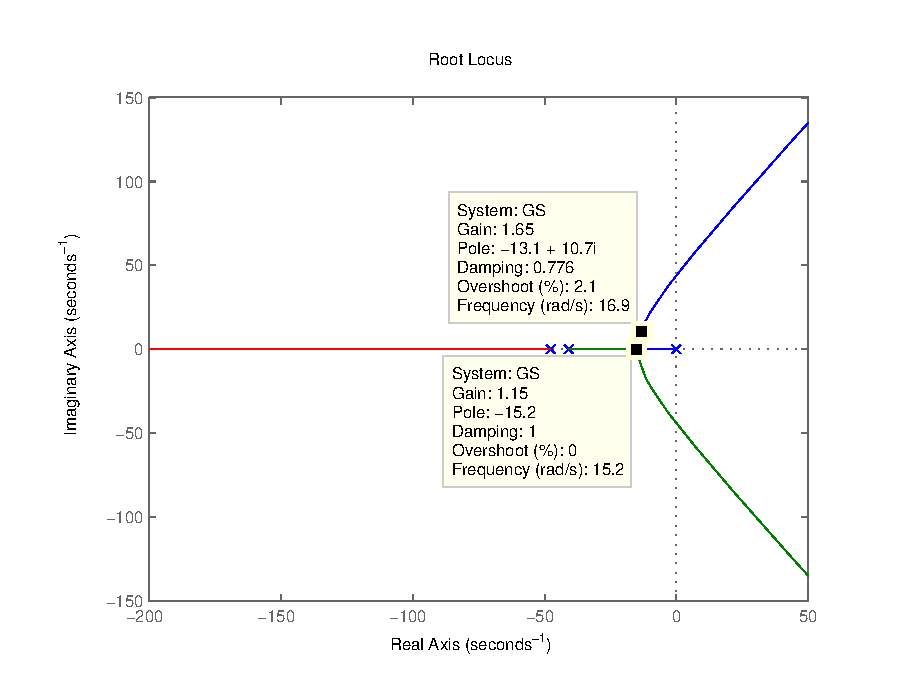
\includegraphics[width=\linewidth]{rlocusgs}
\caption{Diagrama de lugar das raízes para a $G(s)$}
\label{fig:rlocusgs}
\end{figure}
 
 Utilizando as equações fornecidas do \cite{bb:roteiro}:
	\begin{equation}
	\label{eq:establizacao}
	t_{e} = - \frac{ln(\epsilon)}{\xi \omega_n}
	\end{equation}
	\begin{equation}
	\label{eq:overshoot}
	\psi(\xi) = e^{-\frac{\xi\pi}{\sqrt{1-\xi^2}}}
	\end{equation}
	\begin{equation}
	\label{eq:err}
	\epsilon = \lim_{s\to 0} \frac{s}{1 + k*G(s)}*\frac{1}{s^k}
	\end{equation}
 Logo, utilizando os ganhos representados no gráfico calculamos o coeficiente de amortecimento e a frequência natural dos sistemas em malha fechada com o auxílio do Matlab e obtivemos os seguintes valores:
 \begin{itemize}
 	\item{\textbf{Amortecimento crítico}}\\
 	Verificamos o ganho desse item calculando o ponto onde $\frac{k*G(s)}{1 + K*G(S)}$ tem multiplicidade dois, para isso encontramos as raízes $s_1$ e $s_2$ da derivada de $\frac{1}{G(s)}$, substituindo então na relação $k = -\frac{1}{(G(s))}$ encontramos dois valores possíveis para $k$, comparando os valores com os obtidos no diagrama de lugar das raízes, confirmamos o ganho $k = 1.1515$.
	 	Para $\xi = 1$ e $\omega_n = 14.0$ 
	 	 \begin{equation}
	 	 \label{eq:tec}
	 	 t_{e} = 0.28 s
	 	 \end{equation}
	 	 \begin{equation}
	 	 \label{eq:ovc}
	 	 \psi(\xi) = 0
	 	 \end{equation}
	 	 Erro estático da resposta ao degrau:
 	 	 \begin{equation}
 	 	 \label{eq:errcsp}
 	 	 \epsilon = 0
 	 	 \end{equation}
 	 	 Erro estático da resposta a uma rampa:
  	 	 \begin{equation}
  	 	 \label{eq:errcrp}
  	 	 \epsilon = 0.153633
  	 	 \end{equation}
  	\item{\textbf{Sobrelevação de $2\%$}}\\
	  	Com o auxílio do sisotool encontramos o valor para o ponto de sobrelevação $2\%$ com maior precisão, utilizamos então o ganho de $1.6649$ para o controlador.
	  	Para $\xi = 0.776$ e $\omega_n = 17.2$ 
	  	 \begin{equation}
	  	 \label{eq:teo}
	  	 t_{e} = 0.2931 s
	  	 \end{equation}
	 	 \begin{equation}
	 	 \label{eq:ovo}
	 	 \psi(\xi) = 2\%
	 	 \end{equation}
	 	 Erro estático da resposta ao degrau:
	 	 \begin{equation}
	 	 \label{eq:errosp}
	 	 \epsilon = 0
	 	 \end{equation}
	 	 Erro estático da resposta a uma rampa:
	 	 \begin{equation}
	 	 \label{eq:errorp}
	 	 \epsilon = 0.106247
	 	 \end{equation}
 \end{itemize}
 Plotamos então as respostas ao degrau e rampa dos sistemas com cada um dos controladores que podem ser vistas nas figuras \ref{fig:stepgkccl}, \ref{fig:stepgkocl}, \ref{fig:rampgkccl}, \ref{fig:rampgkocl}.
 
 \begin{figure}[H]
 	\centering
 	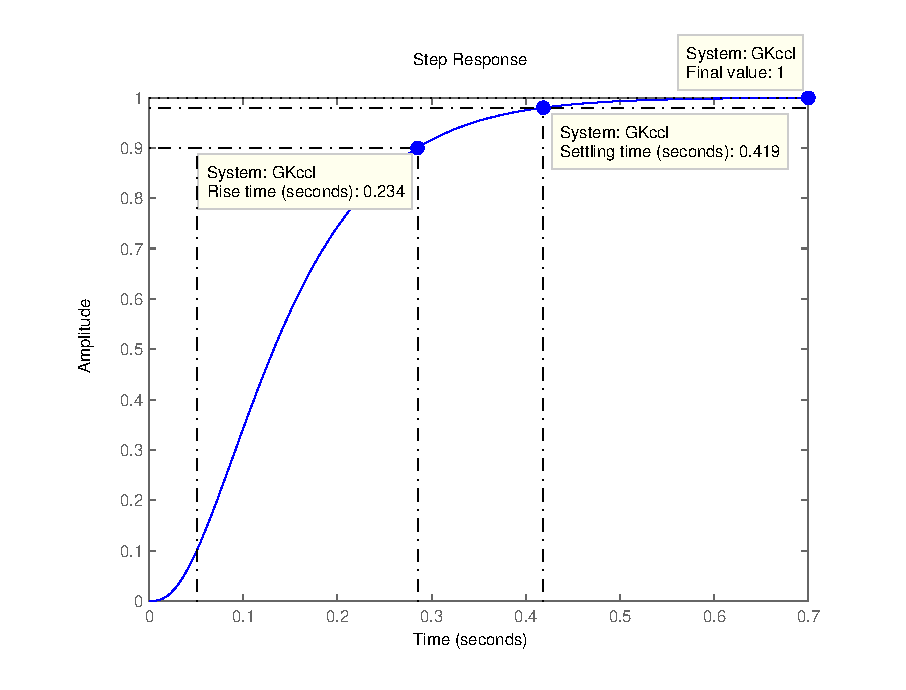
\includegraphics[width=0.8\linewidth]{stepgkccl}
 	\caption{Resposta ao degrau do sistema com controlador projetado para amortecimento crítico}
 	\label{fig:stepgkccl}
 \end{figure}
 
  \begin{figure}[H]
  	\centering
  	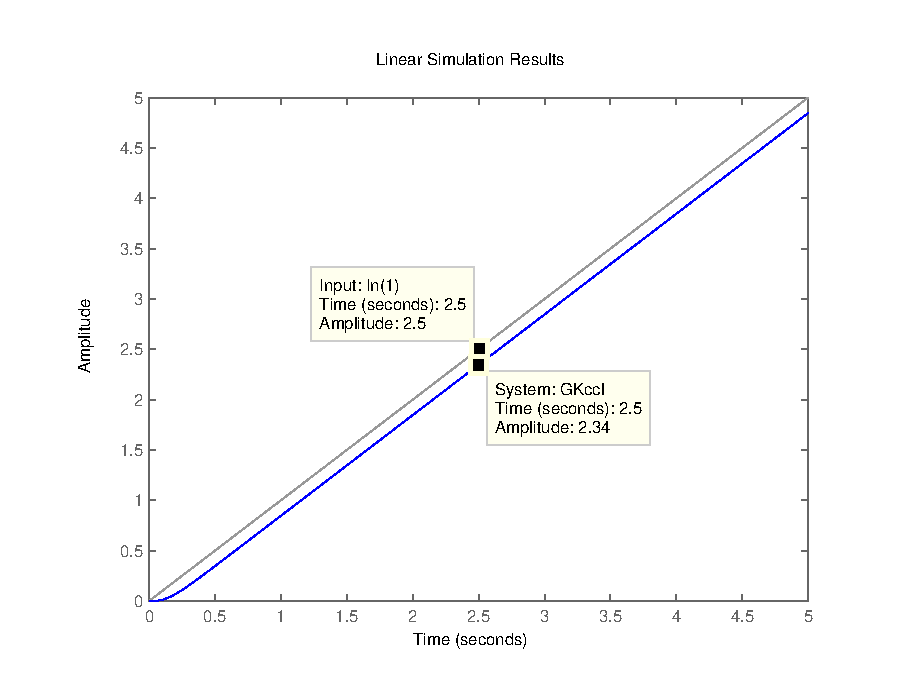
\includegraphics[width=0.8\linewidth]{rampgkccl}
  	\caption{Resposta à rampa do sistema com controlador projetado para amortecimento crítico}
  	\label{fig:rampgkccl}
  \end{figure}
  
   \begin{figure}[H]
   	\centering
   	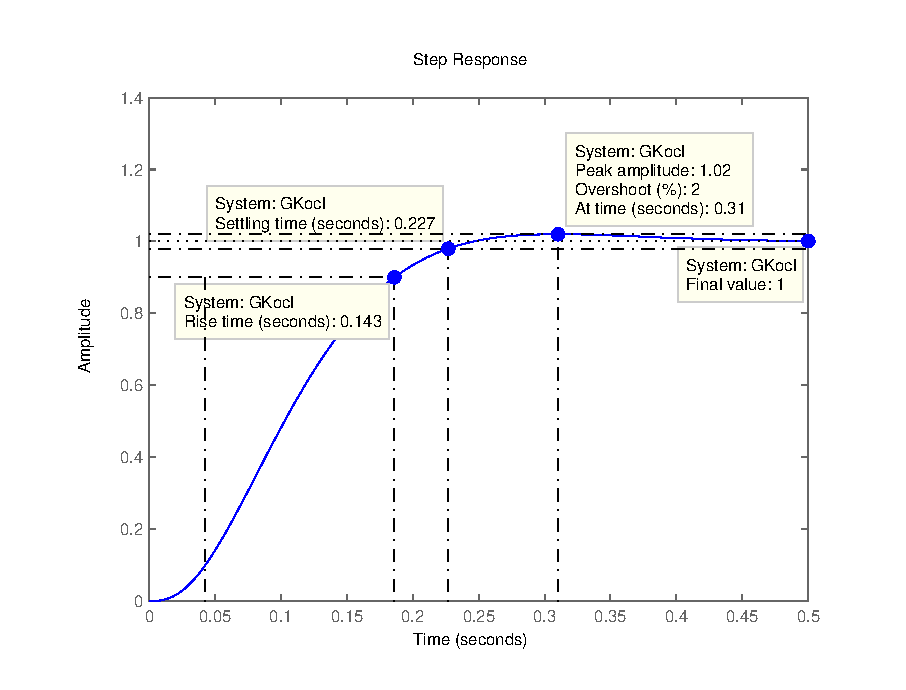
\includegraphics[width=0.8\linewidth]{stepgkocl}
   	\caption{Resposta ao degrau do sistema com controlador projetado para sobrelevação de $2\%$}
   	\label{fig:stepgkocl}
   \end{figure}
   
   \begin{figure}[H]
   	\centering
   	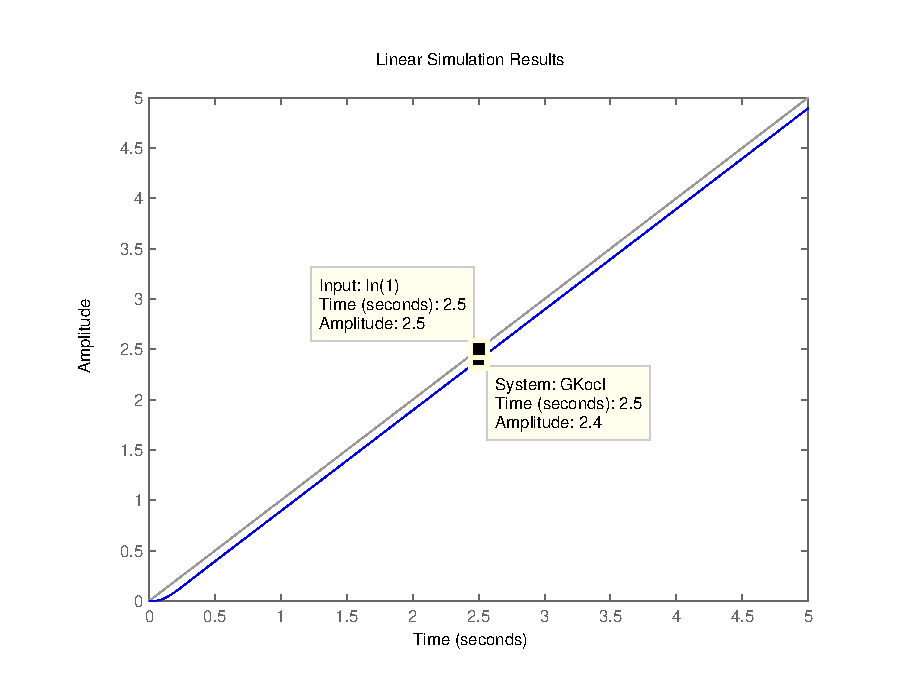
\includegraphics[width=0.8\linewidth]{rampgkocl}
   	\caption{Resposta à rampa do sistema com controlador projetado para sobrelevação de $2\%$}
   	\label{fig:rampgkocl}
   \end{figure}
Comparando os valores calculados, com os obtidos na simulação, podemos perceber que eles são brm próximos, porém ainda existe uma discrepância no tempo de estabilização, isso ocorre devido às aproximações que fizemos durante ao cálculo (só levando em consideração os dois maiores polos) e devido às aproximações que são feitas pelo Matlab durante a simulação do sistema. 
O ponto com amortecimento crítico é o que minimiza a função representada na equação \ref{eq:establizacao}, porém pela simulação, podemos observar que o sistema com sobrelevação de $2\%$ apresenta resultados melhores.

\section{Projeto do controlador PID - Ziegler Nichols}
Através do método de Ziegler Nichols, projetamos um controlador PID $C(s) = k_p*(1 + \frac{1}{T_is} + T_ds)$. Para isto inicialmente plotamos com o auxílio do Matlab o diagrama de lugar das raízes para a planta, que pode ser observado na figura \ref{fig:rlocuslim} encontramos o ponto limite de estabilidade. Também determinamos este ponto utilizando o critério de Routh, obtendo a equação $k_{osc} = \frac{\tau_3 + \tau_2}{\kappa_1*\kappa_2*\kappa_3*\kappa_4*\tau_3*\tau_2)}$ que nos fornece o mesmo valor para $k_{osc}$ de $15.66$.
\begin{figure}[H]
  	\centering
  	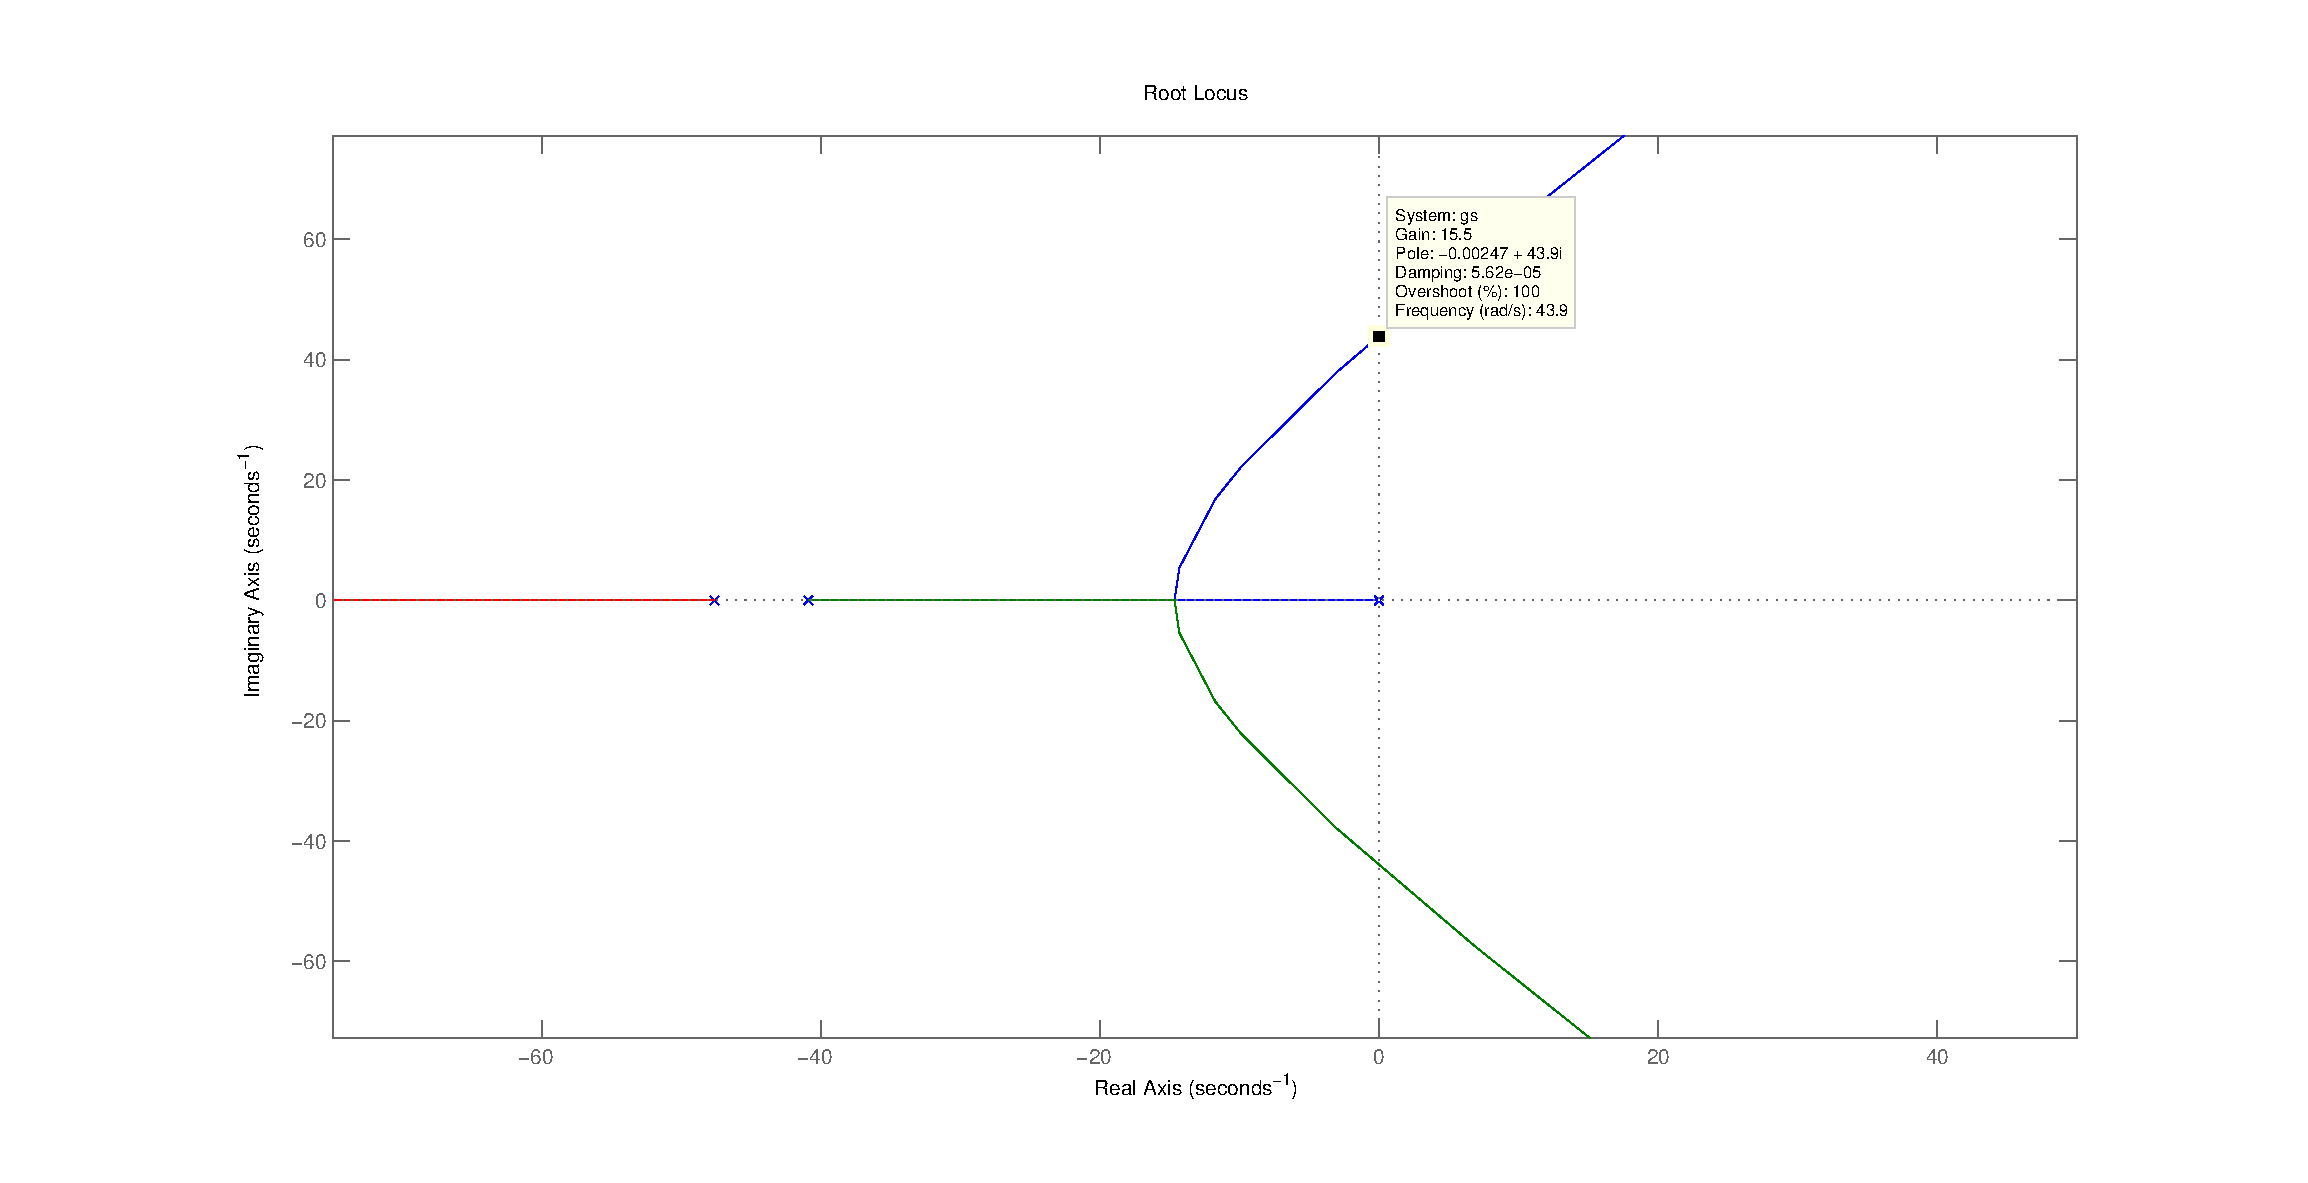
\includegraphics[width=\linewidth]{rlocuslim}
  	\caption{Diagrama de lugar das raízes para a $G(s)$ mostrando o limite de estabilidade}
  	\label{fig:rlocuslim}
\end{figure}
Com esse valor, utilizamos a tabela disponível no roteiro \cite{bb:roteiro} para calcular os parâmetros $T_i = 0.0712$ e $T_d = 0.0178$.
Pelo método do lugar das raízes, tentamos ajustar o valor de $k_p$, porém, como podemos ver na figura \ref{fig:rlocuspidzn} existe uma assíntota que limita o aumento de $\xi \omega_n$ por mais que o ganho $k$ aumente, levando o sistema a ter menor amortecimento (maior sobrelevação) e mesmo tempo de estabilização. Levando em conta essas limitações, escolhemos $k_p = 14$.
\begin{figure}[H]
	\centering
	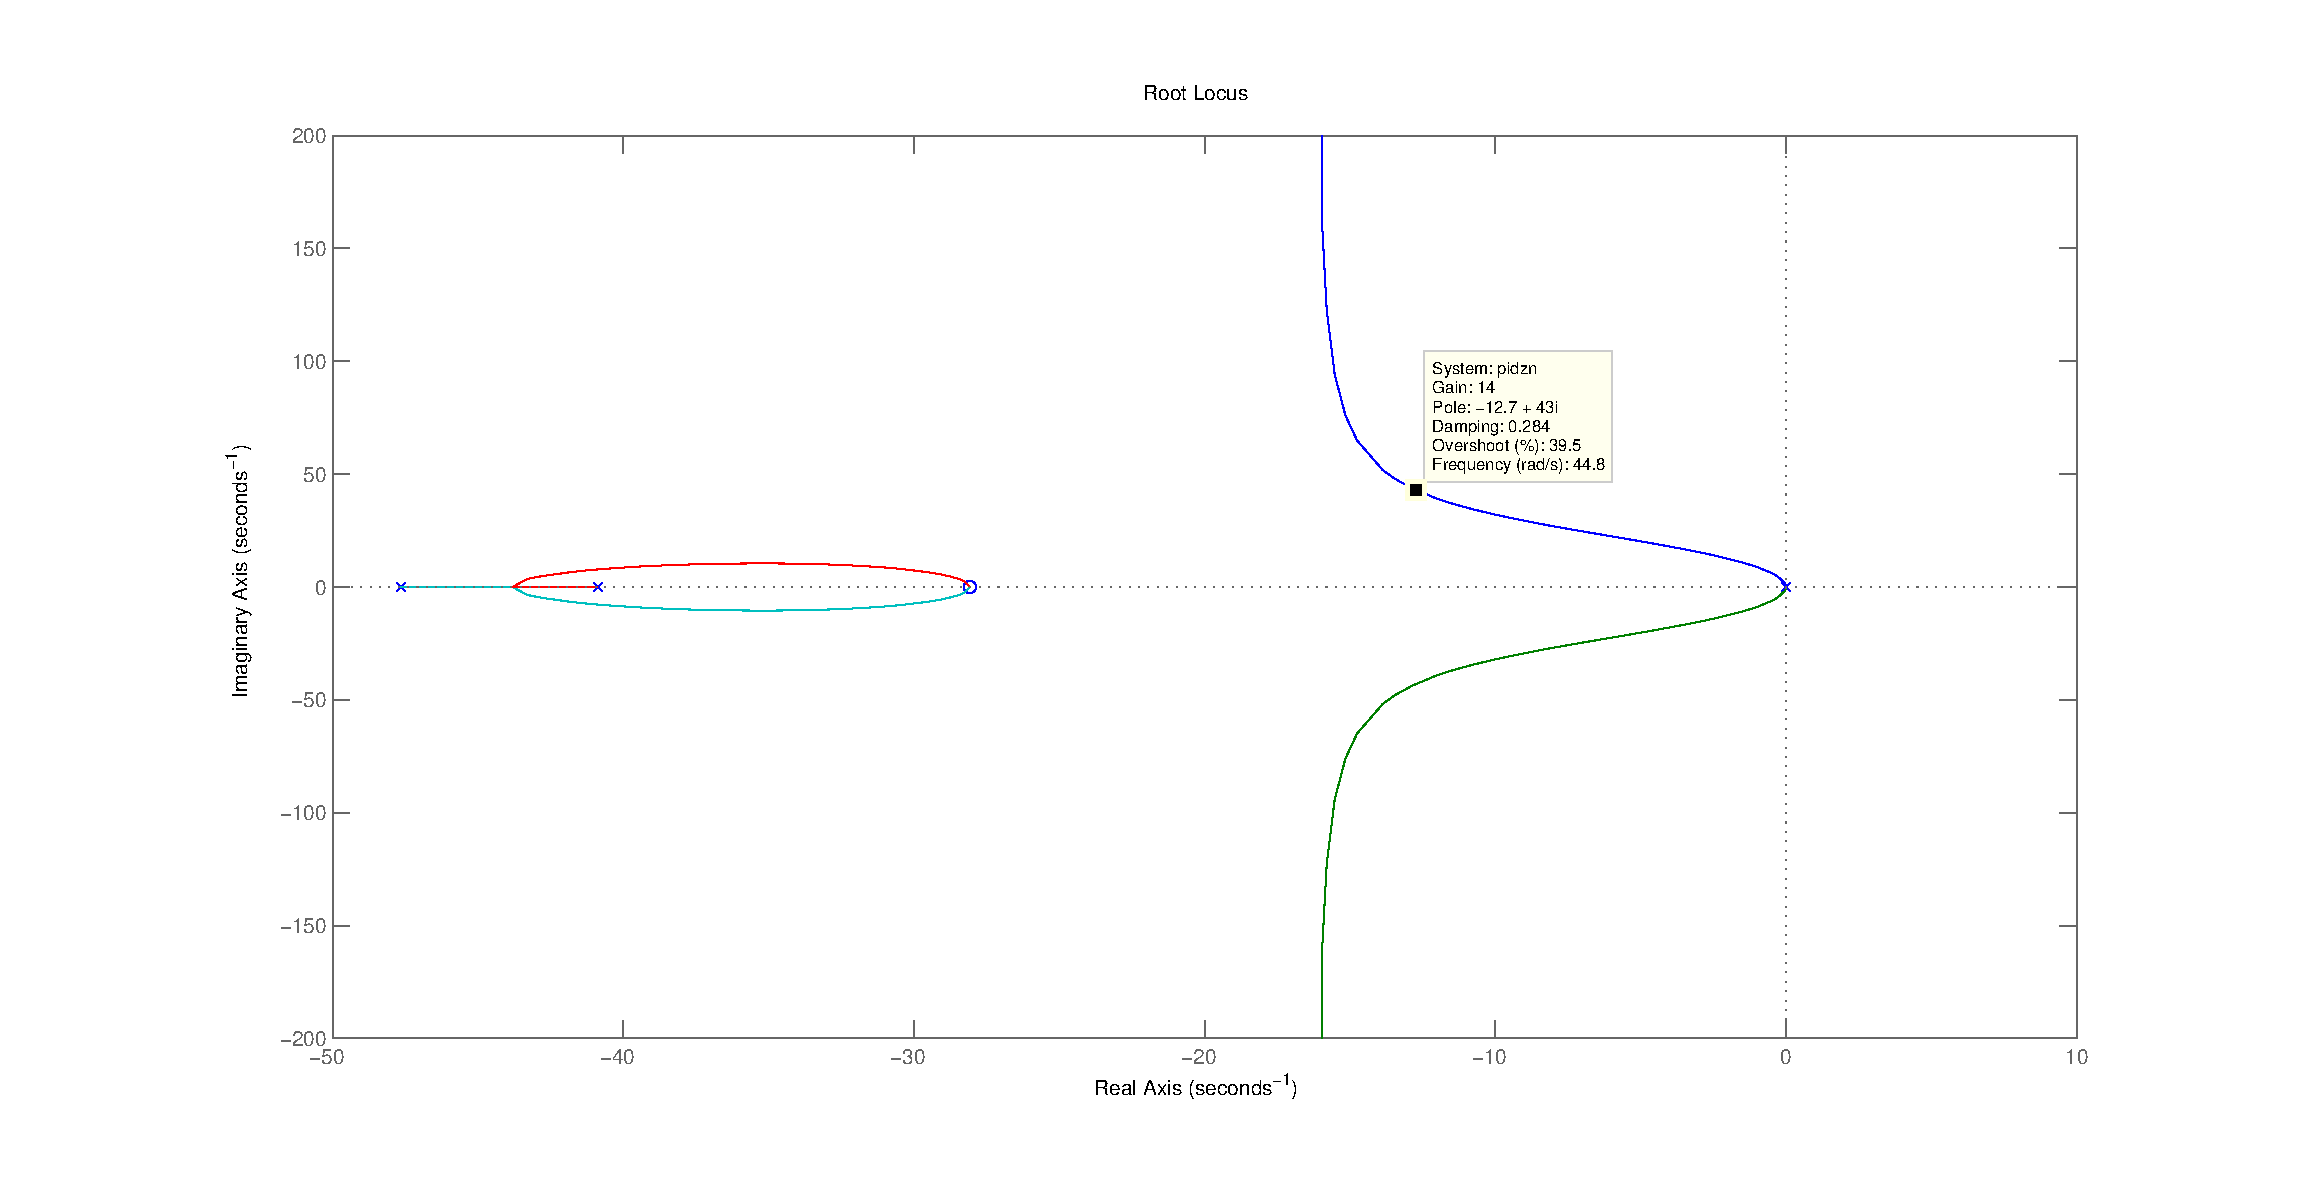
\includegraphics[width=\linewidth]{rlocuspidzn}
	\caption{Diagrama de lugar das raízes para sistema com controlador calculado pelo método de Ziegler-Nichols}
	\label{fig:rlocuspidzn}
\end{figure}

Esse sistema em malha fechada apresenta $\xi = 0.284$ e $\omega_n = 44.8$. Com esses valores e as equações \ref{eq:establizacao}, \ref{eq:overshoot} e \ref{eq:err} calculamos:
		Tempo de estabilização:
	 	 \begin{equation}
	 	 t_{e} = 0.3075 s
	 	 \label{eq:tezn}
	 	 \end{equation}
	 	 Sobrelevação:
	 	 \begin{equation}
	 	 \label{eq:ovzn}
	 	 \psi(\xi) = 39.43\%
	 	 \end{equation}
	 	 Erro estático da resposta ao degrau:
	 	 \begin{equation}
	 	 \label{eq:errznsp}
	 	 \epsilon = 0
	 	 \end{equation}
	 	 Erro estático da resposta à rampa:
	 	 \begin{equation}
	 	 \label{eq:errznrp}
	 	 \epsilon = 0
	 	 \end{equation}
Discretizamos esse controlador por tusting utilizando a função "c2d" do Matlab, com frequência de amostragem de 0.001s. Obtendo a função de transferência discreta:
	\begin{equation}[H]
		C(z) = \frac{518.8 z^2 - 997.1 z + 484.4}{z^2 - 1}
	\end{equation}
	
	\begin{figure}[H]
		\centering
		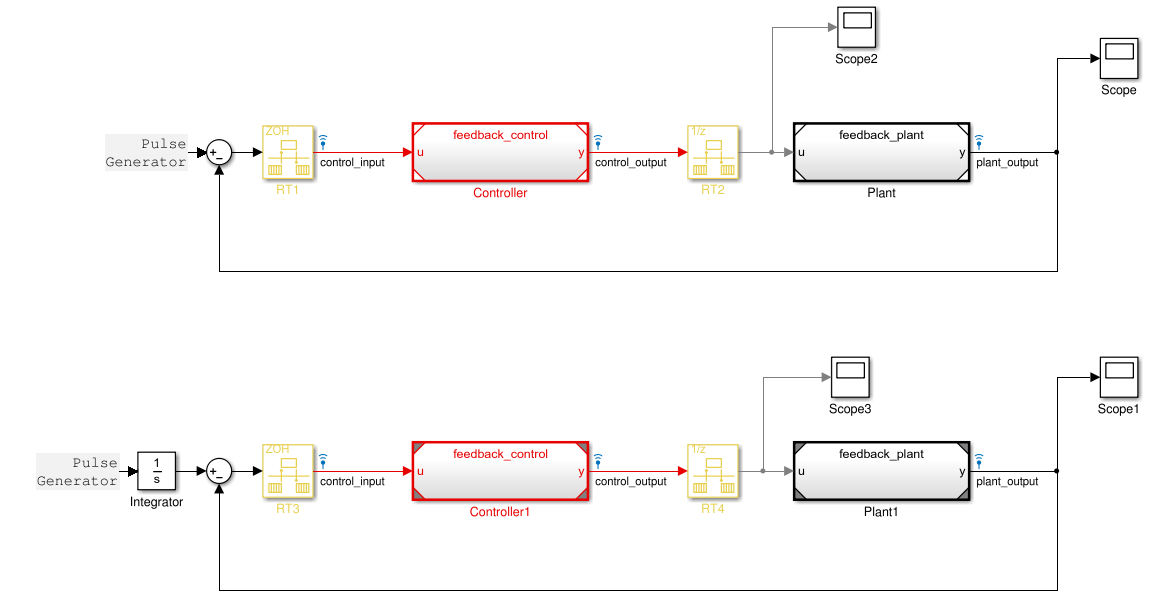
\includegraphics[width=0.8\linewidth]{simulink}
		\caption{Esquema do sistama no simulink}
		\label{fig:simulink}
	\end{figure}
Simulamos o sistema com essa função de transferência no Simulink, como pode ser visto na figura \ref{fig:simulink} e obtivemos como resposta à uma onda quadrada de amplitude $1V$ e frequência $4Hz$ o resultado que pode ser visto nas figuras \ref{fig:stepZN} e \ref{fig:stepuZN} e a resposta à integral dessa onda quadrada (logo uma rampa) pode ser vista nas figuras \ref{fig:rampZN} e \ref{fig:rampuZN}.  
	\begin{figure}[H]
	\centering
	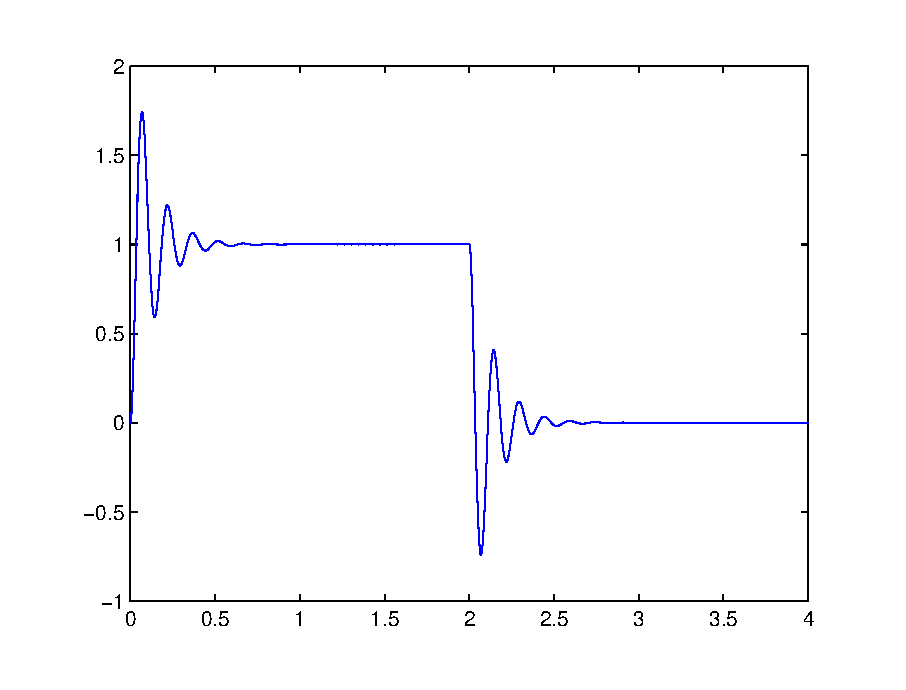
\includegraphics[width=0.8\linewidth]{stepZN}
	\caption{Resposta ($y(t)$) à onda quadrada do sistema com controlador calculado pelo método Ziegler-Nichols discretizado}
	\label{fig:stepZN}
	\end{figure}
	\begin{figure}[H]
	\centering
	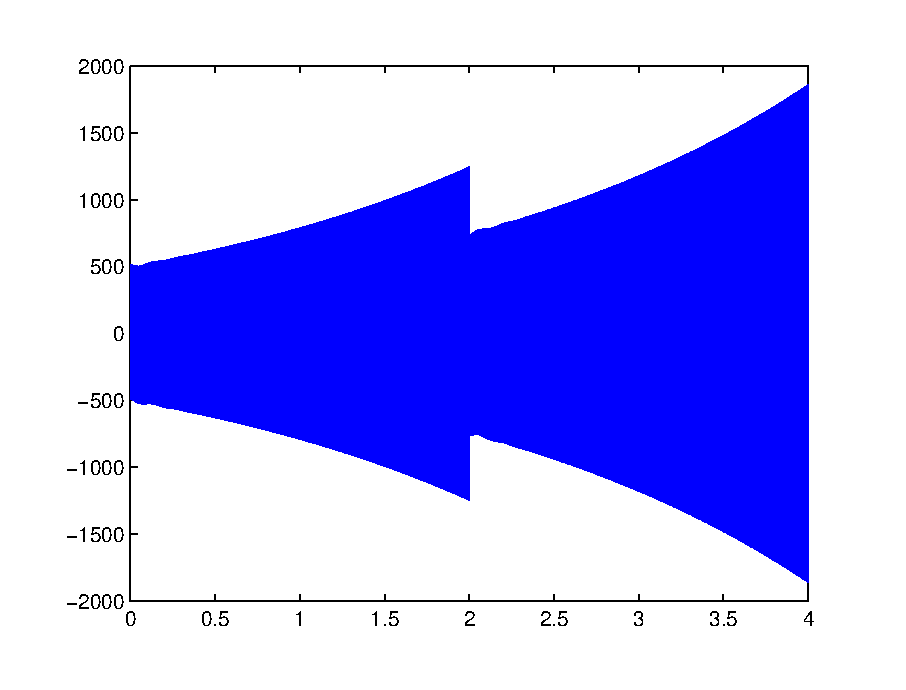
\includegraphics[width=0.8\linewidth]{stepuZN}
	\caption{Esforço de controle ($y(t)$) em resposta a uma onda quadrada do sistema com controlador calculado pelo método Ziegler-Nichols discretizado}
	\label{fig:stepuZN}
	\end{figure}
	\begin{figure}[H]
		\centering
		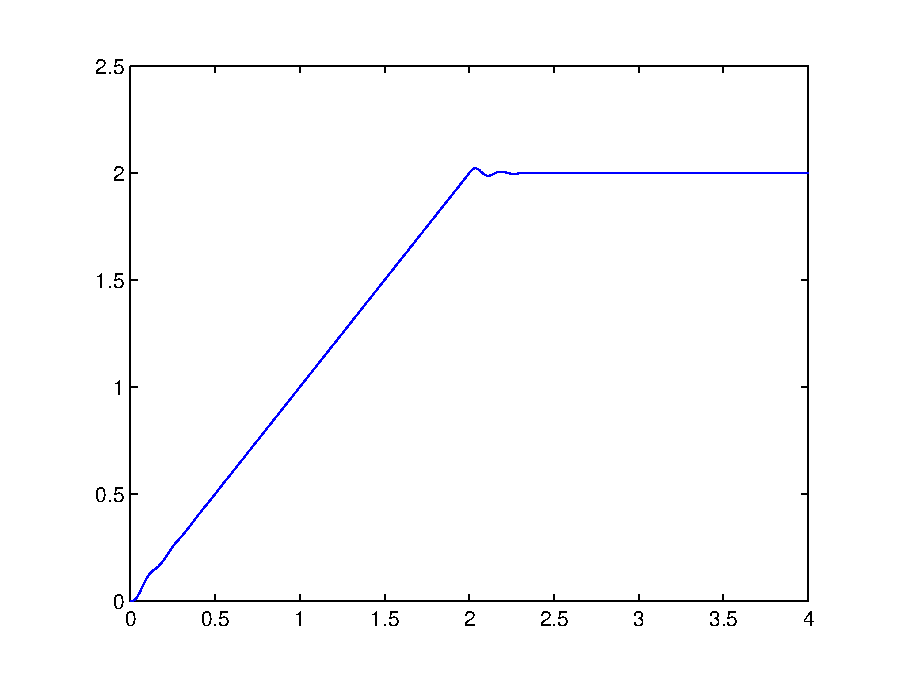
\includegraphics[width=0.8\linewidth]{rampZN}
		\caption{Resposta ($y(t)$) à uma rampa do sistema com controlador calculado pelo método Ziegler-Nichols discretizado}
		\label{fig:rampZN}
	\end{figure}
	\begin{figure}[H]
		\centering
		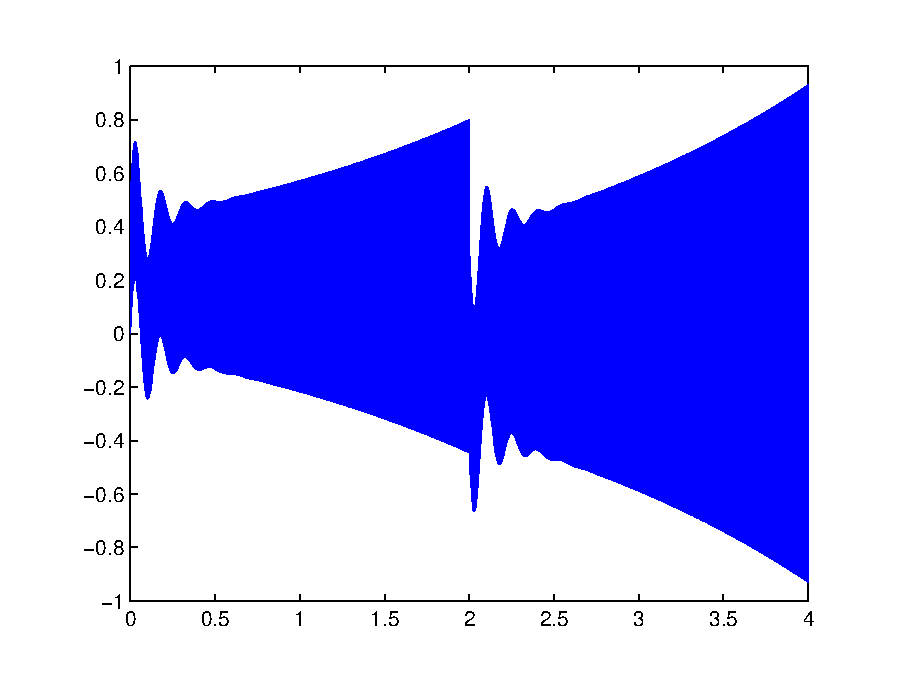
\includegraphics[width=0.8\linewidth]{rampuZN}
		\caption{Esforço de controle ($y(t)$) em resposta à uma rampa do sistema com controlador calculado pelo método Ziegler-Nichols discretizado}
		\label{fig:rampuZN}
	\end{figure}
Como podemos ver, o esforço de controle desse sistema quando discretizado oscila com um período extremamente elevado tornando a sua implementação praticamente impossível. 
Para essas resposta calculamos, com o auxílio da função "stepinfo" do Matlab, os mesmos valores acima e chegamos no resultado:
		Tempo de estabilização:
		\begin{equation}
		t_{e} = 0.24471 s
		\end{equation}
		Sobrelevação:
		\begin{equation}
		\psi(\xi) = 74.19\%
		\end{equation}
		Erro estático da resposta ao degrau:
		\begin{equation}
		\epsilon = 0
		\end{equation}
		Erro estático da resposta à rampa:
		\begin{equation}
		\epsilon = 0.002
		\end{equation}
Notamos que os valores calculados teoricamente são próximos dos medidos durante a simulação, exceto a sobrelevação, essas discrepâncias vêm muito provavelmente da discretização do controlador.
\section{Projeto do controlador PID - Sisotool}
Projetamos o controlador PID para a planta com o auxílio da ferramenta Sisotool do Matlab, e configuramos o método de design para "PID Tuning" e o tipo de controlador para PID, encontrando o controlador $ 11.716*\frac{0.0324s^2 + 0.654s + 1}{0.00017s^2 + s}$. Notamos que um dos polos do controlador foi colocado muito longe da origem conforme apresentado no diagrama de lugar das raízes \ref{fig:rlocusGKs}, e seu efeito no sistema é baixo.
	\begin{figure}[H]
		\centering
		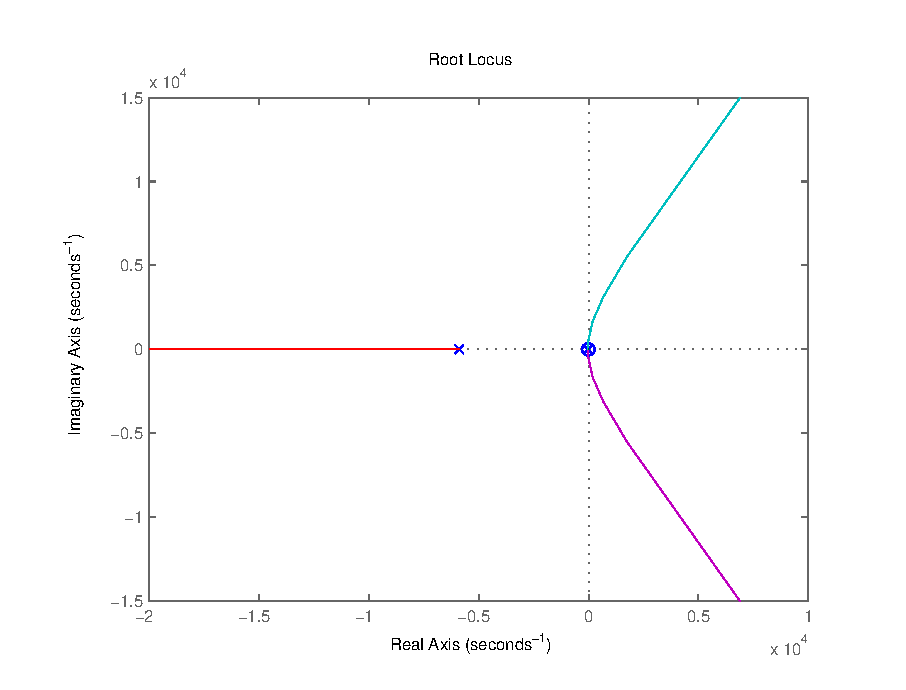
\includegraphics[width=\linewidth]{rlocusGKs}
		\caption{Diagrama de lugar das raízes para sistema com controlador PID projetado com o auxílio do SISOTool}
		\label{fig:rlocusGKs}
	\end{figure}
Para que o tempo de estabilização deste sistema se aproximasse do tempo de estabilização do sistema com o controlador proporcional calculado anteriormente, seu ganho foi alterado para $15.53$, levando seu tempo de estabilização para $0.294$ segundos. Entretanto, outras características como a sobrelevação e tempo de subida não puderam ser reproduzidas, conforme mostrado em \ref{fig:stepgkscl}, e o sistema não apresenta erro à entrada rampa, como podemos ver na \ref{fig:rampgkscl}.
	\begin{figure}[H]
		\centering
		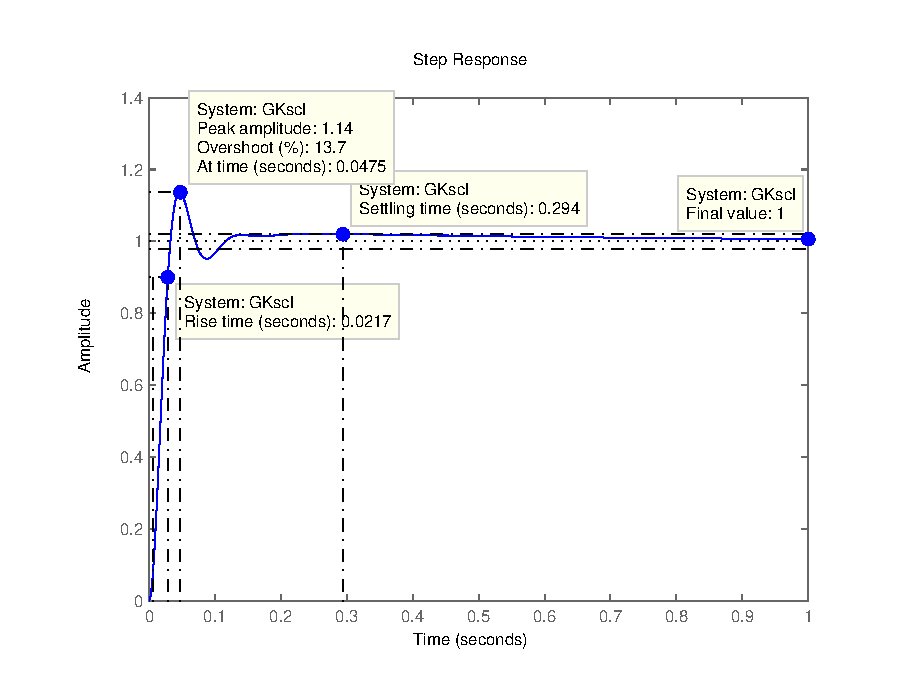
\includegraphics[width=0.8\linewidth]{stepgkscl}
		\caption{Resposta ao degrau para o sistema com controlador PID projetado com o auxílio do SISOTool}
		\label{fig:stepgkscl}
	\end{figure}
	\begin{figure}[H]
		\centering
		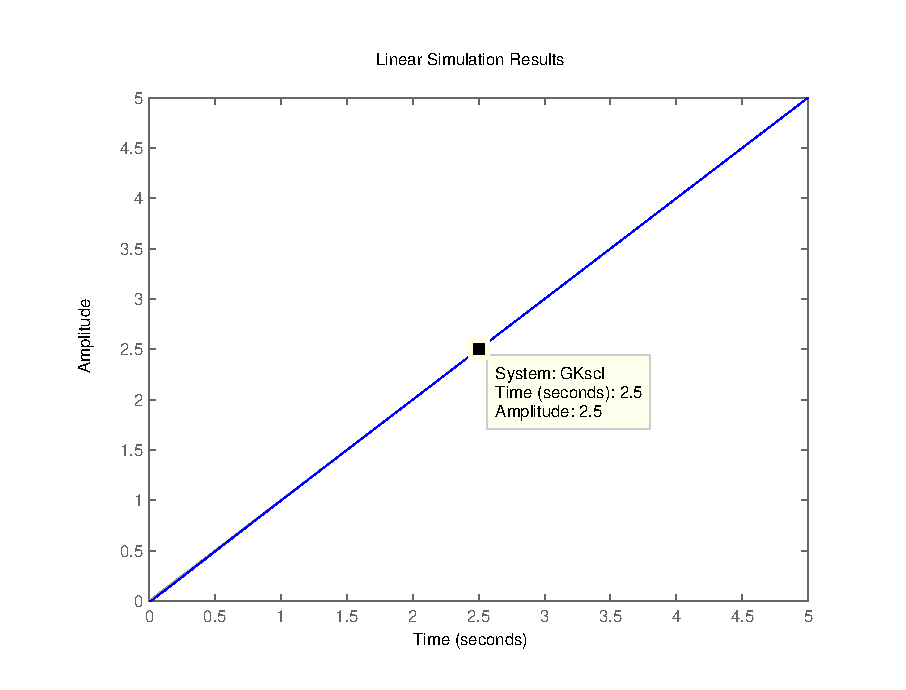
\includegraphics[width=0.8\linewidth]{rampgkscl}
		\caption{Resposta à rampa para o sistema com controlador PID projetado com o auxílio do SISOTool}
		\label{fig:rampgkscl}
	\end{figure}
Para que o sistema tenha tempo de estabilização menor que o sistema com controlador Ziegler Nichols, seu ganho é aumentado para 20, seu tempo de estabilização passa a ser $0.124$ segundos e sua sobrelevação $20\%$, como podemos ver na figura \ref{fig:stepgks2cl}.
	\begin{figure}[H]
		\centering
		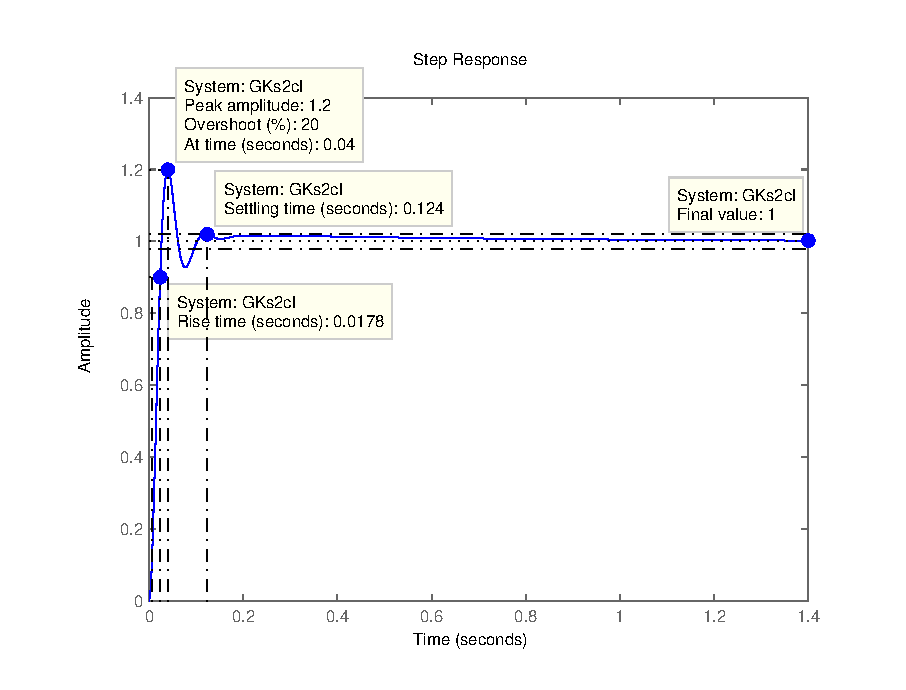
\includegraphics[width=\linewidth]{stepgks2cl}
		\caption{Resposta ao degrau para o sistema com controlador PID projetado com o auxílio do SISOTool}
		\label{fig:stepgks2cl}
	\end{figure}
Utilizando o mesmo método de simulação descrito no projeto do PID Ziegler-Nichols  obtvemos os resultados mostrados nas figuras \ref{fig:stepSISO} e \ref{fig:stepuSISO} e a resposta à integral dessa onda quadrada (logo uma rampa) pode ser vista nas figuras \ref{fig:rampSISO} e \ref{fig:rampuSISO}.  
\begin{figure}[H]
	\centering
	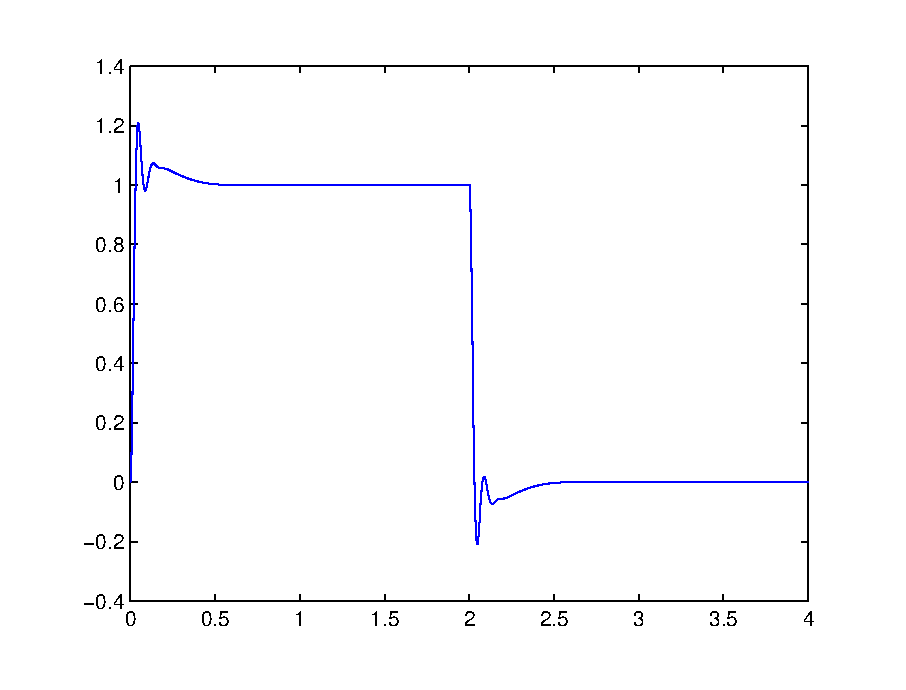
\includegraphics[width=0.8\linewidth]{stepSISO}
	\caption{Resposta ($y(t)$) à onda quadrada do sistema com controlador projetado com o auxílio do SISOTool discretizado}
	\label{fig:stepSISO}
\end{figure}
\begin{figure}[H]
	\centering
	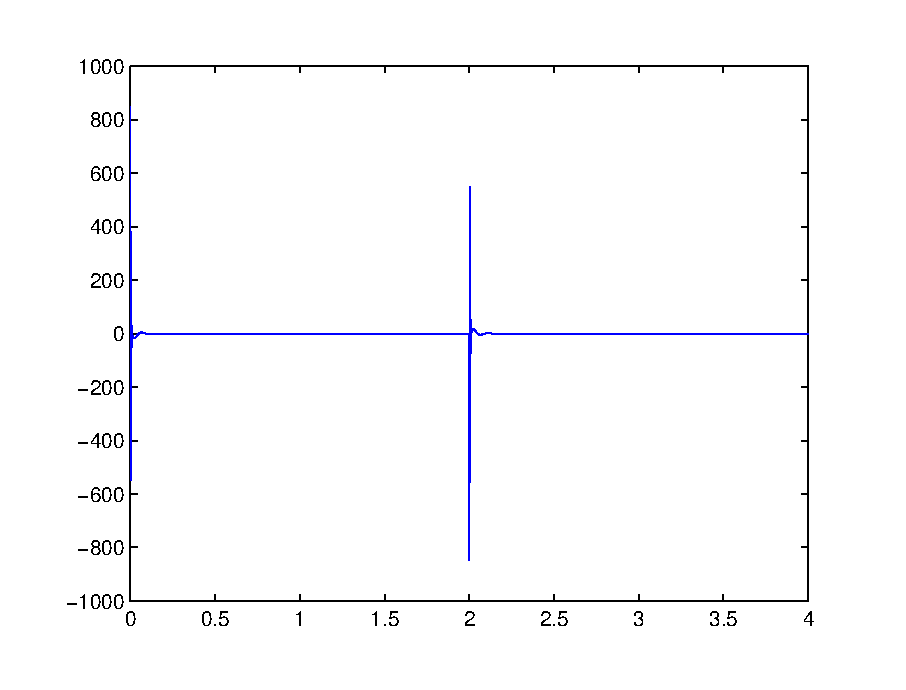
\includegraphics[width=0.8\linewidth]{stepuSISO}
	\caption{Esforço de controle ($y(t)$) em resposta a uma onda quadrada do sistema com controlador projetado com o auxílio do SISOTool discretizado}
	\label{fig:stepuSISO}
\end{figure}
\begin{figure}[H]
	\centering
	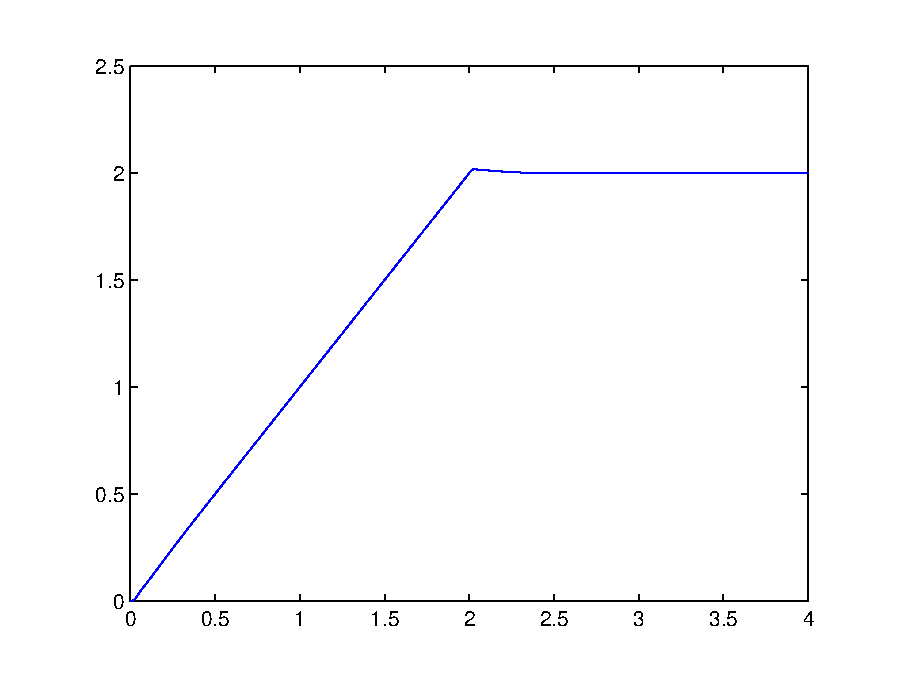
\includegraphics[width=0.8\linewidth]{rampSISO}
	\caption{Resposta ($y(t)$) à uma rampa do sistema com controlador projetado com o auxílio do SISOTool discretizado}
	\label{fig:rampSISO}
\end{figure}
\begin{figure}[H]
	\centering
	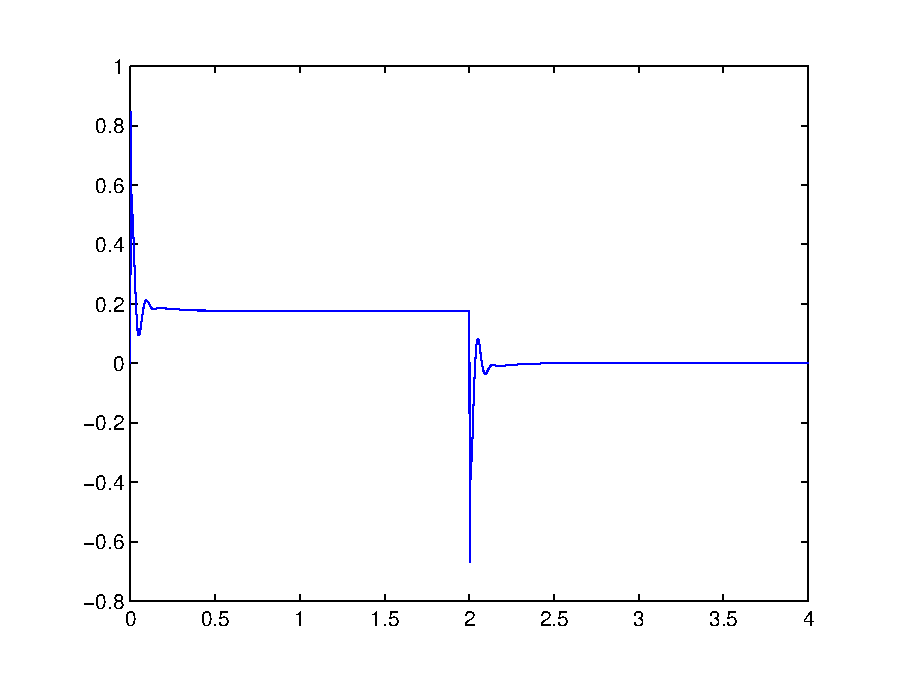
\includegraphics[width=0.8\linewidth]{rampuSISO}
	\caption{Esforço de controle ($y(t)$) em resposta à uma rampa do sistema com controlador projetado com o auxílio do SISOTool discretizado}
	\label{fig:rampuSISO}
\end{figure}
Como podemos ver, o esforço de controle desse sistema na resposta à onda quadrada ultrapassa nosso limiar de 10V, logo acrescentamos um threshold de saturação na simulação, obtendo os resultados das figuras \ref{fig:stepSISOsat} e \ref{fig:stepuSISOsat}
\begin{figure}[H]
	\centering
	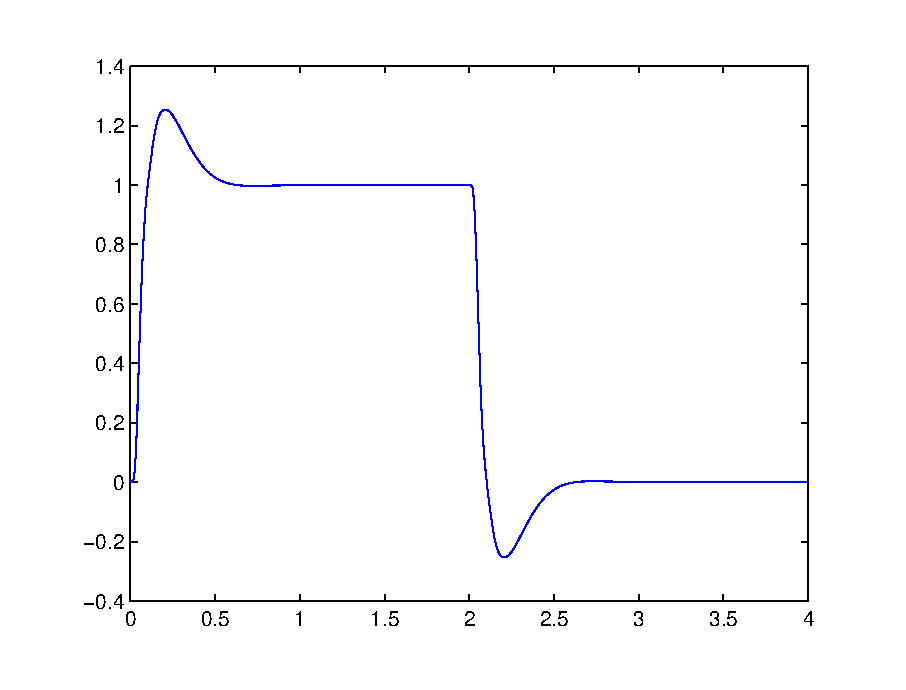
\includegraphics[width=0.8\linewidth]{stepSISOsat}
	\caption{Resposta ($y(t)$) à onda quadrada do sistema com controlador projetado com o auxílio do SISOTool discretizado e com saturação}
	\label{fig:stepSISOsat}
\end{figure}
\begin{figure}[H]
	\centering
	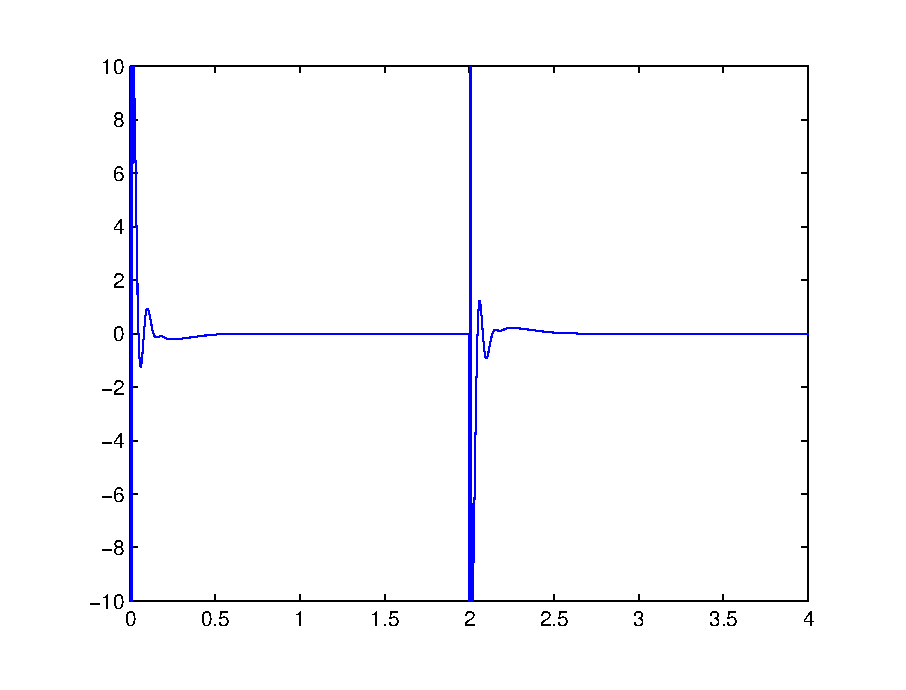
\includegraphics[width=0.8\linewidth]{stepuSISOsat}
	\caption{Esforço de controle ($y(t)$) em resposta a uma onda quadrada do sistema com controlador projetado com o auxílio do SISOTool discretizado e com saturação}
	\label{fig:stepuSISOsat}
\end{figure}
Para essas resposta calculamos, com o auxílio da função "stepinfo" do Matlab, os mesmos valores obtidos nos gráficos acima e chegamos no resultado:
Tempo de estabilização (sem saturação):
\begin{equation}
t_{e} = 0.23306 s
\end{equation}
Tempo de estabilização (com saturação):
\begin{equation}
t_{e} = 0.25010 s
\end{equation}
Sobrelevação (sem saturação):
\begin{equation}
\psi(\xi) = 20.97\%
\end{equation}
Sobrelevação (com saturação):
\begin{equation}
\psi(\xi) = 25.33\%
\end{equation}
Erro estático da resposta ao degrau (sem saturação):
\begin{equation}
\epsilon = 0
\end{equation}
Erro estático da resposta ao degrau (com saturação):
\begin{equation}
\epsilon = 0
\end{equation}
Erro estático da resposta à rampa:
\begin{equation}
\epsilon = 0.002
\end{equation}
Notamos que os valores calculados para o sistema contínuo são próximos dos medidos durante a simulação, com uma pequena diferença que provavelmente provém da discretização do controlador.
Podemos ver que esse controlador tem uma curva de esforço de controle muito mais plausível que o controlador obtido pelo método de Ziegler-Nichols.
	
\begin{thebibliography}{widestlabel}
	\bibitem{bb:roteiro}{Roteiro do experimento disponibilizado para os alunos}
\end{thebibliography}
\end{document}

